Rather than calling it denoising, better word in image reconstruction because
Image Reconstruction:

Purpose: To reconstruct an image from incomplete, noisy, or indirect measurements. This is often used in medical imaging (e.g., MRI, CT scans), computational photography, and computer vision applications. 

Reconstruction involves generating a complete image from partial or indirect data, which can include denoising and deblurring as sub-tasks.

\section{Address reconstruction/denoising schemes}
VST with BM3D
PnP iterative stuff
maybe non local sometime
UNET noise2noise

\section{What is poisson}

\begin{figure}
    \centering
    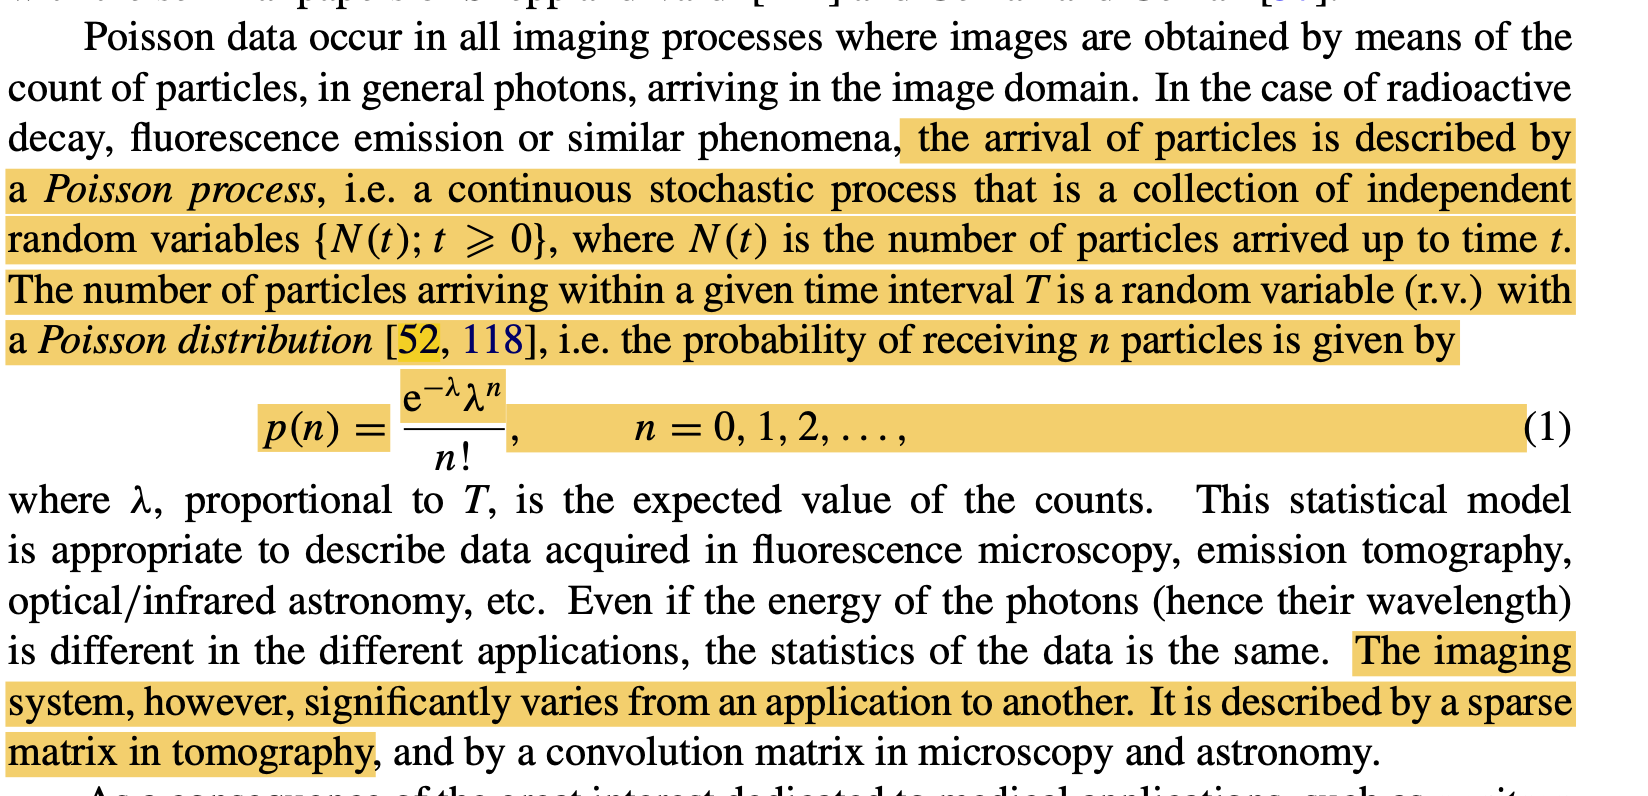
\includegraphics[width=1\linewidth]{JD-54-image.png}
    \caption{Enter Caption}
    \label{fig:enter-label}
\end{figure}

Taken from \cite{Bertero2009} which cites \cite{Feller1968-mq}

\section{Testing process for poisson}
To determine if your images (or the events they represent) are coming from a Poisson process, you need to perform statistical tests that check for the key characteristics of a Poisson process. A Poisson process has the following properties:

1. **Events occur independently**: The occurrence of one event does not affect the probability of another event occurring.
2. **Constant rate ($\lambda$)**: The average number of events in a given time interval is constant.
3. **No simultaneous events**: Two events cannot occur at the exact same time.

### Steps to Test if Images Come from a Poisson Process

1. **Estimate the Rate ($\lambda$):**
Calculate the average rate at which events (images) occur over time. This is the mean number of events per unit time.
2. **Check for Independence:**
Ensure that the events occur independently. This can be tested using:
    - **Inter-arrival times**: The times between consecutive events should follow an exponential distribution if the events are Poisson-distributed.
3. **Statistical Tests:**
    - **Chi-Square Goodness-of-Fit Test**: Compare the observed distribution of counts in intervals to the expected distribution under the Poisson assumption.
    - **Kolmogorov-Smirnov (K-S) Test**: Compare the distribution of inter-arrival times to the exponential distribution.

### Detailed Steps

1. **Calculate Inter-arrival Times:**
    - Compute the time intervals between consecutive events (images).
    - Plot a histogram of these inter-arrival times and compare it to the exponential distribution with rate \( λ \).
2. **Perform the Kolmogorov-Smirnov Test:**
    
    ```python
    from scipy.stats import kstest, expon
    import numpy as np
    
    # Assume `inter_arrival_times` is a list or array of the inter-arrival times
    inter_arrival_times = np.diff(event_times)  # event_times is the array of event timestamps
    λ = 1 / np.mean(inter_arrival_times)  # Mean rate
    
    # Perform K-S test
    D, p_value = kstest(inter_arrival_times, 'expon', args=(0, 1/λ))
    print("K-S Test statistic:", D)
    print("p-value:", p_value)
    
    ```
    
    - A high p-value (typically > 0.05) indicates that you cannot reject the hypothesis that the inter-arrival times follow an exponential distribution.
3. **Chi-Square Goodness-of-Fit Test:**
    - Divide the observation period into equal intervals.
    - Count the number of events in each interval.
    - Compare the observed counts to the expected counts under the Poisson distribution.
    
    ```python
    from scipy.stats import chisquare
    
    # Assume `counts` is the array of event counts in each interval
    interval_length = ...  # Define the length of each interval
    observed_counts = np.histogram(event_times, bins=np.arange(0, max(event_times) + interval_length, interval_length))[0]
    expected_counts = [λ * interval_length] * len(observed_counts)  # λ * length of the interval
    
    chi2, p_value = chisquare(observed_counts, expected_counts)
    print("Chi-Square statistic:", chi2)
    print("p-value:", p_value)
    
    ```
    
    - A high p-value (typically > 0.05) indicates that you cannot reject the hypothesis that the counts follow a Poisson distribution.

### Interpretation

If your tests show that:

- The inter-arrival times follow an exponential distribution (high p-value in K-S test).
- The counts in intervals follow a Poisson distribution (high p-value in Chi-Square test).

Then you have evidence that your images are coming from a Poisson process.

### What Does a Poisson Process Mean?

A Poisson process is a stochastic process that models a series of events occurring randomly over time, with the following characteristics:

- **Randomness and Independence**: Each event occurs independently of the others.
- **Constant Average Rate**: Events occur at a constant average rate \( λ \).
- **Memorylessness**: The time until the next event is independent of the time since the last event, following an exponential distribution.

This kind of process is useful for modeling random events over time, such as arrivals of customers, radioactive decay, or image captures in surveillance.

By confirming that your images are from a Poisson process, you validate the assumption that the events they represent occur randomly and independently at a constant average rate.

